\chapter{ऊष्मा चालन}\label{ch:b2:heat-conduction}

किसी एक ठंडी सुबह धातु की पटरी और लकड़ी की बेंच को छूकर देखिए: पटरी अधिक
ठंडी लगती है, हालाँकि कोई तापमापी दोनों को वही ताप देता है। चूल्हे पर कोई
कड़ाही रखिए और उसका हत्था कुछ देर बाद ही गरम होता है; गर्मियों में दो मीटर
खोदिए और मिट्टी सर्दी की ठंड लिए बैठी है; और कोई प्रोसेसर जो किसी वर्ग
सेंटीमीटर पर सौ वाट व्यय करता है इसलिए नहीं पिघलता क्योंकि उस पर
पंखियों वाला ऐलुमिनियम का कोई गुटका बैठा है। यह सब \emph{ऊष्मा चालन} है,
अर्थात् अणुओं की उथल-पुथल से पदार्थ में होकर आंतरिक ऊर्जा का परिवहन, बिना
पदार्थ के किसी बहाव के --- और यह सब एक ही नियम, फ़ूरिये वाले, और एक ही
समीकरण, ऊष्मा समीकरण, को मानता है, जो पिछले अध्याय का \omterm{thm:b2:particle-diffusion:equation}{विसरण समीकरण} ही है,
घनत्व की जगह ताप के साथ। यह अध्याय नियम और समीकरण को किसी ऊर्जा-संतुलन से
खड़ा करता है, उन्हें उन हालों में हल करता है जो मायने रखते हैं (स्थायी
दीवारें और उनके \omterm{prop:b2:heat-conduction:resistance}{तापीय प्रतिरोध}, आवर्ती तापन तथा तापीय तरंग, शीतलक पंखियाँ),
किसी तरल के साथ विनिमय बताता है (न्यूटन का नियम और \omterm{def:b2:heat-conduction:biot}{बायो संख्या}), और वह
एंट्रॉपी निकालता है जो चालन बनाता है --- क्योंकि ऊष्मा केवल ढलान पर ही बहती है।

\begin{omfigure}
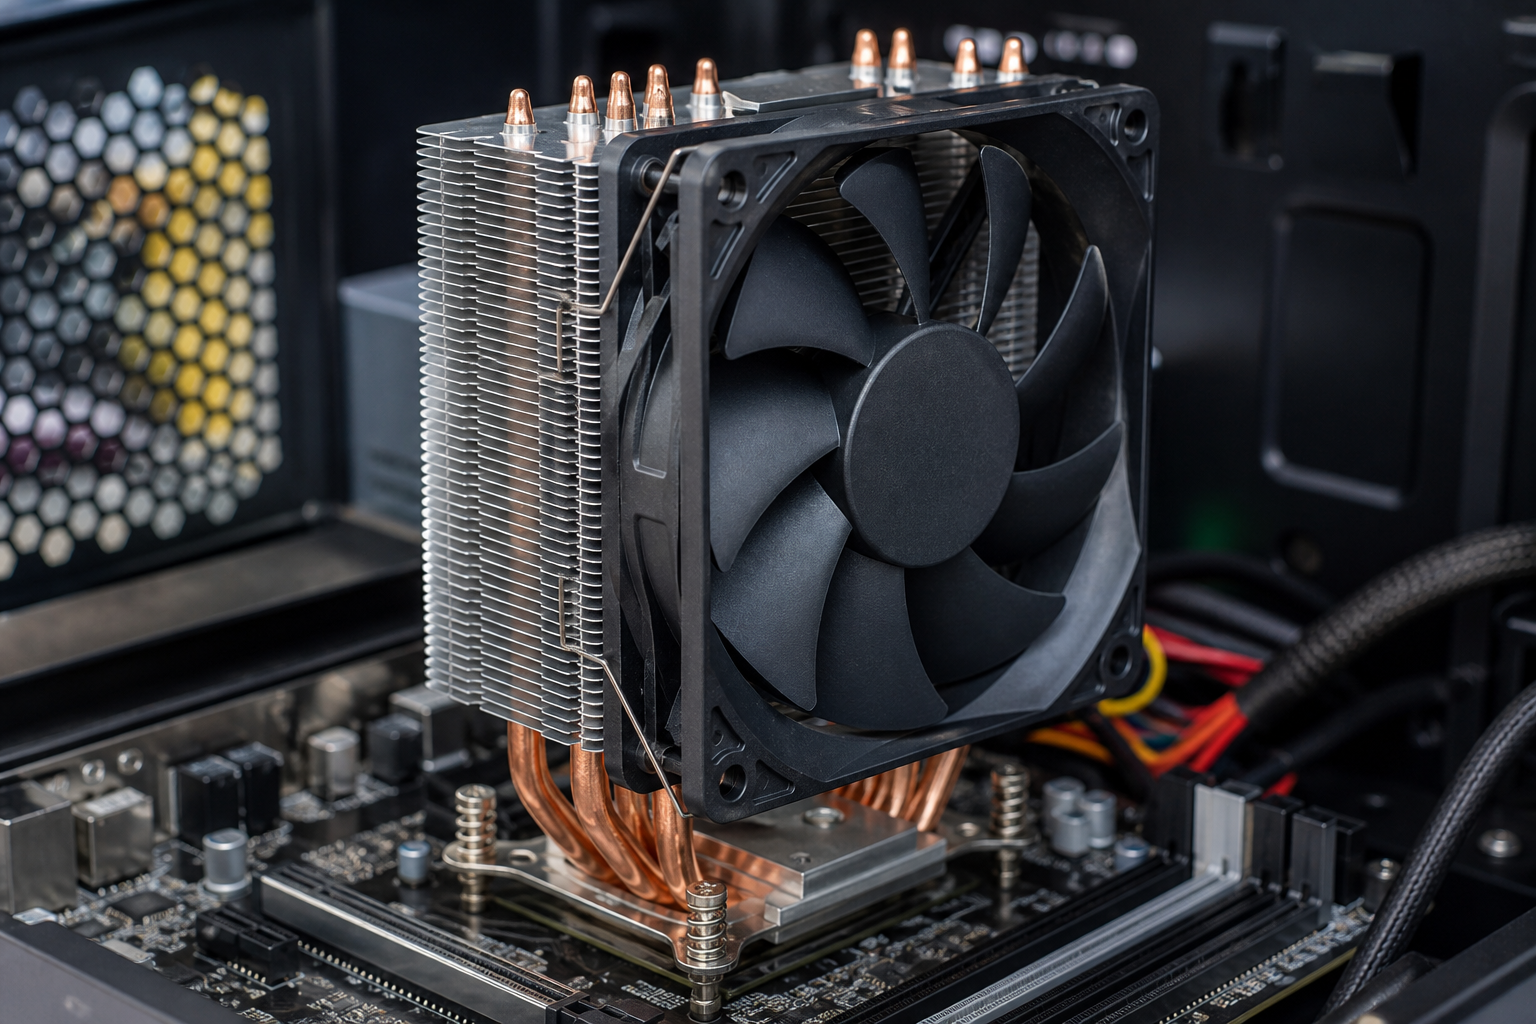
\includegraphics[width=0.58\linewidth]{images/book4/ai/b4-25-cpu-heat-sink.png}

{\small किसी प्रोसेसर पर पंखियों वाला कोई ऊष्मा-अपसारक: सिलिकॉन के किसी वर्ग
सेंटीमीटर से बाहर चालित सौ वाट, जो धातु के किसी आधार भर फैलाए जाते हैं,
और उन पंखियों से हवा को सौंप दिए जाते हैं जो सतह को तीस गुना कर देती हैं।}
\end{omfigure}

\section{फ़ूरिये का नियम}

\begin{definition}[ऊष्मा धारा-घनत्व]\label{def:b2:heat-conduction:flux}
\emph{ऊष्मा धारा-घनत्व}\index{ऊष्मा धारा-घनत्व}
$\vect{j}_Q$ (\unit{W/m^2} में) वह सदिश है जिसके लिए किसी दिष्ट सतह-अवयव
$\dd\vect S$ से होकर $\dd t$ के दौरान चालन से
अंतरित ऊर्जा $\vect{j}_Q\cdot\dd\vect S\,\dd t$ हो; और किसी
सतह $S$ से होकर \emph{तापीय फ्लक्स}\index{तापीय फ्लक्स} (कोई शक्ति, वाट में)
$\Phi = \iint_S\vect{j}_Q\cdot\dd\vect S$ है।
\end{definition}

\begin{theorem}[फ़ूरिये का नियम]\label{thm:b2:heat-conduction:fourier}
विरामावस्था के किसी माध्यम में, जिसका ताप एकसमान न हो,
\[
\vect{j}_Q = -\lambda\,\vect{\operatorname{grad}}\,T ,
\]
जहाँ \emph{तापीय चालकता}\index{तापीय चालकता}
$\lambda > 0$ (\unit{W/m/K} में) पदार्थ पर और, दुर्बल रूप से,
ताप पर निर्भर करती है। ऊष्मा ताप की \omterm{def:b2:maxwell-equations:operators}{प्रवणता} से नीचे बहती है, गरम से
ठंडे की ओर --- अर्थात् किसी रैखिक नियम में गुँथा दूसरा नियम।
\end{theorem}

\begin{proof}
परिघटनात्मक, फ़िक के नियम की तरह, और उसी सूक्ष्म
औचित्य के साथ: अणु (या किसी धातु के मुक्त इलेक्ट्रॉन, या
जालक के कंपन) अपनी ऊर्जा किसी यादृच्छिक चाल पर ले चलते हैं, और उसमें से अधिक
गरम पक्ष से आती है।
\end{proof}

\begin{example}[चालकताएँ]\label{ex:b2:heat-conduction:values}
धातुएँ (इलेक्ट्रॉन ऊष्मा भी वैसे ही ले चलते हैं जैसे धारा ---
और चालकताएँ एक-दूसरे के पीछे चलती हैं): ताँबा \qty{400}{W/m/K}, ऐलुमिनियम
\qty{240}{W/m/K}, इस्पात \qty{50}{W/m/K}। विद्युतरोधी ठोस: कंक्रीट
\qty{1.5}{W/m/K}, काँच \qty{1}{W/m/K}, ईंट \qty{0.8}{W/m/K}, लकड़ी
\qty{0.15}{W/m/K}। द्रव: जल \qty{0.6}{W/m/K}। गैसें: हवा
\qty{0.026}{W/m/K} --- और सबसे अच्छे विद्युतरोधी, \qty{0.04}{W/m/K} पर
काँच की ऊन या झाग, अधिकतर ठहरी हुई हवा ही हैं, इस तरह फँसाई गई कि वह
संवहन न कर सके। ताँबे से हवा तक चार कोटियाँ।
\end{example}

\section{ऊर्जा-संतुलन और ऊष्मा समीकरण}

\begin{theorem}[स्थानीय ऊर्जा-संतुलन]\label{thm:b2:heat-conduction:balance}
घनत्व $\rho$ और विशिष्ट ऊष्मा $c$ के किसी ठोस में (या विरामावस्था के किसी
तरल में), जहाँ प्रति एकांक आयतन शक्ति $p$ छूटती हो (जूल तापन, कोई
रासायनिक या नाभिकीय अभिक्रिया, सोखा गया विकिरण),
\[
\rho c\,\frac{\partial T}{\partial t} = -\operatorname{div}\vect{j}_Q + p ,
\qquad\text{एक विमा में}\quad
\rho c\,\frac{\partial T}{\partial t} = -\frac{\partial j_Q}{\partial x} + p .
\]
\end{theorem}

\begin{proof}
$x$ और $x + \dd x$ के बीच के पट्ट के लिए पहला नियम (\omterm{prop:b2:laser:gain}{अनुप्रस्थ काट} $S$,
नियत आयतन, अतः कोई कार्य नहीं): उसकी आंतरिक ऊर्जा $\rho c\,T\,S\,\dd x$
$\dd t$ में पाई गई ऊष्मा से बदलती है, $[j_Q(x) - j_Q(x+\dd x)]S\,\dd t
= -\partial_x j_Q\,\dd x\,S\,\dd t$, और साथ में $p\,S\,\dd x\,\dd t$। तीन
विमाओं में किसी नियत आयतन में उसकी बंद सतह से होकर आती ऊष्मा
$-\iint\vect{j}_Q\cdot\dd\vect S = -\iiint\operatorname{div}\vect{j}_Q\,\dd\tau$ है।
\end{proof}

\begin{theorem}[ऊष्मा समीकरण]\label{thm:b2:heat-conduction:equation}
एकसमान $\lambda$, $\rho$, $c$ के लिए,
\[
\frac{\partial T}{\partial t} = a\,\Delta T + \frac{p}{\rho c},
\qquad a = \frac{\lambda}{\rho c} \quad\text{(\emph{तापीय विसरणता}\index{तापीय विसरणता}, \unit{m^2/s} में)} .
\]
\omterm{thm:b2:particle-diffusion:equation}{विसरण समीकरण} के बारे में जो कुछ कहा गया वह सब टिका रहता है: रैखिकता,
अनुत्क्रमणीयता, चिकनाना, और पैमाने $L \sim \sqrt{at}$, $t \sim
L^2/a$।
\end{theorem}

\begin{proof}
संतुलन में फ़ूरिये का नियम डालिए: $\rho c\,\partial_t T =
\lambda\Delta T + p$।
\end{proof}

\begin{example}[विसरणताएँ और काल]\label{ex:b2:heat-conduction:times}
ताँबा $a = \qty{1.1e-4}{m^2/s}$, हवा \qty{2e-5}{m^2/s}, कंक्रीट और
ईंट $\approx \qty{5e-7}{m^2/s}$, जल \qty{1.4e-7}{m^2/s}, लकड़ी
\qty{1e-7}{m^2/s}। ऊष्मा ताँबे का कोई सेंटीमीटर किसी सेकंड में पार करती है, ईंट का
कोई सेंटीमीटर तीन मिनट में, \qty{20}{cm} की कोई दीवार किसी दिन में
(और इसीलिए मोटी दीवारें दिन--रात के चक्र को चिकना कर देती हैं), किसी स्टेक की
\qty{1.5}{cm} अर्ध-मोटाई घंटे के चौथाई में (पकाने के
काल मोटाई के वर्ग की तरह बदलते हैं), और चट्टान का कोई किलोमीटर
$10^{12}\,\unit{s}$ में, यानी तीस हज़ार वर्ष --- अर्थात् पृथ्वी अब भी अपने
बनने से ठंडी होती जा रही है।
\end{example}

\section{स्थायी दशा: तापीय प्रतिरोध}

\begin{proposition}[किसी पट्ट का तापीय प्रतिरोध]\label{prop:b2:heat-conduction:resistance}
बिना स्रोतों की स्थायी दशा में, मोटाई $e$, क्षेत्रफल $S$,
चालकता $\lambda$ का कोई पट्ट, तापों $T_1$ और
$T_2$ के बीच, कोई रैखिक परिच्छेद रखता है और यह फ्लक्स ले चलता है
\[
\Phi = \frac{T_1 - T_2}{R_{\text{ताप}}}, \qquad
R_{\text{ताप}} = \frac{e}{\lambda S}\quad\text{(\unit{K/W} में)} :
\]
अर्थात् उसका \emph{तापीय प्रतिरोध}\index{तापीय प्रतिरोध}। ताप
विभव की भूमिका निभाता है, और फ्लक्स धारा की: श्रेणी में प्रतिरोध
(किसी दीवार की परतें) जुड़ते हैं, और समांतर में (दीवार और
खिड़की) उनके व्युत्क्रम जुड़ते हैं। त्रिज्याओं $r_1 < r_2$ के बीच और लंबाई $\ell$
के किसी बेलनाकार खोल (किसी नल का विद्युतरोधन) के लिए,
$R_{\text{ताप}} = \ln(r_2/r_1)/2\pi\lambda\ell$; और किसी गोलीय खोल के लिए,
$(1/r_1 - 1/r_2)/4\pi\lambda$।
\end{proposition}

\begin{proof}
$\dd^2T/\dd x^2 = 0$: एकघाती परिच्छेद, $j_Q = \lambda(T_1 - T_2)/e$
एकसमान, $\Phi = j_QS$। बेलनाकार ज्यामिति में $\Phi = -\lambda\,2\pi
r\ell\,\dd T/\dd r$ हर $r$ पर वही है (कोई संचय नहीं), अतः
$T = A - (\Phi/2\pi\lambda\ell)\ln r$; और गोलीय ज्यामिति में $\Phi =
-4\pi r^2\lambda\,\dd T/\dd r$ देता है $T = A + \Phi/4\pi\lambda r$।
\end{proof}

\begin{proposition}[किसी तरल के साथ विनिमय: न्यूटन का नियम]\label{prop:b2:heat-conduction:newton}
$T_{\text{सतह}}$ पर कोई ठोस सतह, जो $T_{\text{तरल}}$ पर किसी तरल के संपर्क में हो
(सतह से दूर), यह फ्लक्स-घनत्व खोती है
\[
j_Q = h\,(T_{\text{सतह}} - T_{\text{तरल}}) ,
\]
जहाँ \emph{ऊष्मा-अंतरण गुणांक}\index{ऊष्मा-अंतरण
गुणांक} $h$ (\unit{W/m^2/K} में) दीवार से चिपकी तरल की पतली परत से
चालन और उसे नया करते संवहन, दोनों को समेट लेता है:
प्राकृतिक या हलके संवहन में हवा के लिए $h \approx 5$--\qty{25}{W/m^2/K},
प्रणोदित हवा के लिए $50$--\qty{500}{W/m^2/K}, और जल के लिए $10^3$--$10^4$।
तब सतह दीवार के साथ श्रेणी में कोई \emph{झिल्ली प्रतिरोध} $1/hS$ जोड़ देती है।
\end{proposition}

\begin{proof}
परिघटनात्मक: तरल की गति निकाली नहीं जाती, उसे
$h$ में समेट दिया जाता है (नापकर, या तरल यांत्रिकी के सहसंबंधों से)।
\end{proof}

\begin{omfigure}
\begin{tikzpicture}[scale=0.9, >=stealth]
  % wall layers
  \fill[omExo!15] (0,0) rectangle (1.6,2.6);
  \fill[omDef!12] (1.6,0) rectangle (2.6,2.6);
  \fill[gray!15] (2.6,0) rectangle (2.8,2.6);
  \draw (0,0) rectangle (2.8,2.6);
  \draw (1.6,0) -- (1.6,2.6); \draw (2.6,0) -- (2.6,2.6);
  \node[font=\scriptsize] at (0.8,2.85) {ईंट};
  \node[font=\scriptsize] at (2.1,2.85) {ऊन};
  \node[font=\scriptsize, right] at (2.9,1.3) {भीतर $T_{\text{भीतर}}$};
  \node[font=\scriptsize, left] at (-0.1,1.3) {बाहर $T_{\text{बाहर}}$};
  \draw[->, omThm, thick] (3.6,0.7) -- (-0.8,0.7) node[midway, below, font=\scriptsize] {$\Phi$};
  % resistor chain
  \begin{scope}[yshift=-1.6cm]
    \draw (-0.8,0) -- (0.2,0);
    \draw (0.2,-0.18) rectangle (1.0,0.18); \node[font=\tiny] at (0.6,0) {$1/h_{\text{बाहर}}S$};
    \draw (1.0,0) -- (1.4,0);
    \draw (1.4,-0.18) rectangle (2.4,0.18); \node[font=\tiny] at (1.9,0) {$e_1/\lambda_1 S$};
    \draw (2.4,0) -- (2.8,0);
    \draw (2.8,-0.18) rectangle (3.8,0.18); \node[font=\tiny] at (3.3,0) {$e_2/\lambda_2 S$};
    \draw (3.8,0) -- (4.2,0);
    \draw (4.2,-0.18) rectangle (5.0,0.18); \node[font=\tiny] at (4.6,0) {$1/h_{\text{भीतर}}S$};
    \draw (5.0,0) -- (5.6,0);
    \fill (-0.8,0) circle (1.5pt) node[above, font=\scriptsize] {$T_{\text{बाहर}}$};
    \fill (5.6,0) circle (1.5pt) node[above, font=\scriptsize] {$T_{\text{भीतर}}$};
  \end{scope}
  % profile
  \begin{scope}[xshift=7.2cm]
    \draw[->] (0,0) -- (3.4,0) node[right, font=\scriptsize] {$x$};
    \draw[->] (0,0) -- (0,2.8) node[above, font=\scriptsize] {$T$};
    \draw[omDef, thick] (0,0.4) -- (0.3,0.6) -- (1.6,0.9) -- (2.6,2.4) -- (2.8,2.45) -- (3.2,2.6);
    \draw[dashed] (0.3,0) -- (0.3,0.6); \draw[dashed] (1.6,0) -- (1.6,0.9); \draw[dashed] (2.6,0) -- (2.6,2.4); \draw[dashed] (2.8,0) -- (2.8,2.45);
    \node[font=\scriptsize, below] at (0.95,0) {ईंट};
    \node[font=\scriptsize, below] at (2.1,0) {ऊन};
    \node[font=\scriptsize, left] at (0,0.4) {$T_{\text{बाहर}}$};
    \node[font=\scriptsize, right] at (3.2,2.6) {$T_{\text{भीतर}}$};
  \end{scope}
\end{tikzpicture}

{\small कोई मिश्रित दीवार और उसका तापीय परिपथ: झिल्ली, ईंट, ऊन,
झिल्ली, श्रेणी में। दाएँ: ताप का परिच्छेद --- लगभग पूरी गिरावट
सबसे बड़े प्रतिरोध वाली परत, यानी ऊन, पर पड़ती है, हालाँकि वही
सबसे पतली है।}
\end{omfigure}

\begin{example}[कोई दीवार और कोई खिड़की]\label{ex:b2:heat-conduction:wall}
प्रति वर्ग मीटर: \qty{0.8}{W/m/K} पर \qty{20}{cm} ईंट, $R =
\qty{0.25}{m^2.K/W}$; और दोनों झिल्लियाँ, $1/8 + 1/25 = \qty{0.165}{m^2.K/W}$:
कुल $0.415$, अर्थात् $U = 1/R = \qty{2.4}{W/m^2/K}$ और, \qty{20}{K}
के अंतर के लिए, \qty{48}{W/m^2}। काँच की ऊन के \qty{10}{cm} जोड़िए, $R =
\qty{2.5}{m^2.K/W}$: कुल $2.9$ हो जाता है, $U = \qty{0.34}{W/m^2/K}$ ---
यानी सात गुना कम। काँच का कोई अकेला फलक, \qty{1}{W/m/K} पर \qty{4}{mm},
पूरा झिल्ली ही है: $R = 0.004 + 0.165$, $U \approx \qty{6}{W/m^2/K}$; और दो
फलकों के बीच ठहरी हवा की \qty{12}{mm} परत $0.012/0.026 =
\qty{0.46}{m^2.K/W}$ जोड़ देती है तथा हानि को तीन से भी अधिक से भाग देती है।
\end{example}

\begin{definition}[बायो संख्या]\label{def:b2:heat-conduction:biot}
किसी तरल के साथ विनिमय करते आकार $L$ के किसी ठोस के लिए, \emph{बायो
संख्या}\index{बायो संख्या}
\[
\mathrm{Bi} = \frac{hL}{\lambda} = \frac{\text{भीतरी प्रतिरोध } L/\lambda S}{\text{झिल्ली प्रतिरोध } 1/hS}
\]
दोनों की तुलना करती है। यदि $\mathrm{Bi} \ll 1$ हो तो ठोस हर क्षण ताप में
एकसमान रहता है और पूरा-का-पूरा, समय-अचर $\tau = \rho c V/hS$ के साथ चरघातांकी
रूप से ठंडा होता है; और यदि $\mathrm{Bi} \gg 1$ हो तो
सतह तरल के ताप पर होती है और भीतरी भाग अपनी ही
चाल $L^2/a$ से चालन करता है।
\end{definition}

\section{आवर्ती तापन: तापीय तरंग}

\begin{proposition}[किसी अर्ध-आकाश में तापीय तरंग]\label{prop:b2:heat-conduction:wave}
यदि किसी अर्ध-आकाश की सतह $x = 0$ को $T(0,t) = T_0 +
\theta_0\cos\omega t$ पर थामा जाए, तो भीतर ताप, जमी हुई
दशा में, है
\[
T(x,t) = T_0 + \theta_0\,\eu^{-x/\delta}\cos\Big(\omega t - \frac{x}{\delta}\Big),
\qquad \delta = \sqrt{\frac{2a}{\omega}} :
\]
अर्थात् कोई तरंग जो भीतर की ओर चाल $\omega\delta =
\sqrt{2a\omega}$ से चलती है और कला के प्रति रेडियन किसी एक \emph{प्रवेश गहराई} $\delta$
भर अवमंदित होती है --- अर्थात् प्रति तरंगदैर्घ्य $\eu^{-2\pi} = 2 \times 10^{-3}$ से।
तेज़ दोलन धीमों से कम घुसते हैं।
\end{proposition}

\begin{proof}
$\underline T = \theta_0\eu^{\iu(\omega t - \underline k x)}$ खोजिए:
$\iu\omega = -a\underline k^2$, अतः $\underline k^2 = -\iu\omega/a$,
$\underline k = (1 - \iu)\sqrt{\omega/2a} = (1 - \iu)/\delta$ (वह मूल
जो $x > 0$ के लिए क्षय करता है)। वास्तविक भाग लीजिए।
\end{proof}

\begin{omfigure}
\begin{tikzpicture}
  \begin{axis}[omaxis, width=9cm, height=4.8cm, xmin=0, xmax=4.6, ymin=-1.1, ymax=1.1,
    xlabel={$x/\delta$}, ylabel={$(T - T_0)/\theta_0$}, xtick={1,2,3,4}, ytick={-1,1}, clip=false,
    axis x line=middle, axis y line=left,
    legend style={font=\scriptsize, at={(0.98,0.04)}, anchor=south east, draw=none, fill=none}]
    \addplot[omDef, thick, domain=0:4.6, samples=120] {exp(-x)*cos(deg(-x))};
    \addlegendentry{$\omega t = 0$}
    \addplot[omThm, thick, domain=0:4.6, samples=120] {exp(-x)*cos(deg(pi/2-x))};
    \addlegendentry{$\omega t = \pi/2$}
    \addplot[omExo, thick, domain=0:4.6, samples=120] {exp(-x)*cos(deg(pi-x))};
    \addlegendentry{$\omega t = \pi$}
    \addplot[gray, dashed, domain=0:4.6, samples=60] {exp(-x)};
    \addplot[gray, dashed, domain=0:4.6, samples=60] {-exp(-x)};
  \end{axis}
\end{tikzpicture}

{\small तीन क्षणों पर तापीय तरंग: सतह का दोलन
किसी अवमंदित तरंग की तरह घुसता है, जिसका आयाम $\eu^{-x/\delta}$ की तरह गिरता है
(बिंदुदार) और जिसकी कला $x/\delta$ से पिछड़ती है --- और $x = \pi\delta$ पर
ताप सतह वाले के उलट होता है।}
\end{omfigure}

\begin{example}[मिट्टी, तहख़ाना और शराब]\label{ex:b2:heat-conduction:soil}
मिट्टी, $a \approx \qty{5e-7}{m^2/s}$। दैनिक चक्र, $\omega = 2\pi/\qty{86400}{s}$:
$\delta = \qty{12}{cm}$ --- आधा मीटर नीचे दिन ग़ायब है। वार्षिक चक्र:
$\delta = \qty{2.2}{m}$; उस गहराई पर गर्मी--सर्दी का \qty{10}{K} का झूला
घटकर \qty{3.7}{K} रह जाता है और एक रेडियन, यानी दो महीने, पिछड़ जाता है: अतः तहख़ाना
मार्च में सबसे ठंडा और सितंबर में सबसे गरम होता है, और \qty{5}{m} पर वह
अचर से \qty{1}{K} दूर है --- वही तहख़ाना जो शराब सँभालता है। वही
गणित विद्युत्चुंबकत्व की \omterm{def:b2:dispersion-wave-packets:complex}{त्वचा गहराई} देता है
(\cref{ch:b2:waves-in-media}): वही समीकरण, वही $\sqrt{2/(\text{विसरणता}
\times\omega)}$।
\end{example}

\section{पंखियाँ}

\begin{proposition}[शीतलक पंखी]\label{prop:b2:heat-conduction:fin}
कोई पतली छड़ या पट्टिका (\omterm{prop:b2:laser:gain}{अनुप्रस्थ काट} $S$, परिमाप $p$, चालकता $\lambda$),
जो $x = 0$ पर $T_0$ की किसी दीवार से जुड़ी हो, $T_{\text{तरल}}$ के किसी तरल में,
गुणांक $h$ के साथ, आधिक्य ताप $\theta = T - T_{\text{तरल}}$
रखती है जो यह मानता है
\[
\frac{\dd^2\theta}{\dd x^2} = m^2\theta, \qquad m = \sqrt{\frac{hp}{\lambda S}} ;
\]
किसी लंबी पंखी के लिए, $\theta = \theta_0\eu^{-mx}$ और पंखी $\Phi =
\sqrt{hp\lambda S}\,\theta_0$ बाहर निकाल देती है --- अर्थात् उतना ही जितना $\sqrt{\lambda
S/hp} = 1/m$ लंबी कोई नंगी सतह, और ताप गिरकर $\theta_0/\eu$ रह जाता है
$x = 1/m$ पर। परिमित लंबाई $L$ की किसी पंखी के लिए (नोक रुद्धोष्म), $\theta =
\theta_0\cosh m(L-x)/\cosh mL$ और उसकी \emph{दक्षता}\index{पंखी की
दक्षता} --- अर्थात् फ्लक्स बटा $\theta_0$ पर किसी समतापी पंखी का फ्लक्स ---
$\eta = \tanh(mL)/mL$ है।
\end{proposition}

\begin{proof}
$[x, x + \dd x]$ फाँक का स्थायी संतुलन: भीतर चालित,
$-\lambda S\theta'(x)$; बाहर, $-\lambda S\theta'(x + \dd x)$; और तरल को
खोया, $hp\,\theta\,\dd x$: $\lambda S\theta'' = hp\theta$। तली पर
फ्लक्स $-\lambda S\theta'(0)$ है: लंबी पंखी के लिए $\lambda Sm\theta_0$,
और परिमित के लिए $\lambda Sm\theta_0\tanh mL$, जिसकी तुलना
$hpL\theta_0$ से करनी है। और एकविमीय निर्वाह के लिए पंखी की मोटाई भर
\omterm{def:b2:heat-conduction:biot}{बायो संख्या}, $ht/\lambda$, छोटी होनी चाहिए।
\end{proof}

\begin{omfigure}
\begin{tikzpicture}
  \begin{axis}[omaxis, width=6.4cm, height=4.4cm, xmin=0, xmax=3.2, ymin=0, ymax=1.12,
    xlabel={$mx$}, ylabel={$\theta/\theta_0$}, xtick={1,2,3}, ytick={1}, clip=false,
    legend style={font=\scriptsize, at={(0.98,0.98)}, anchor=north east, draw=none, fill=none}]
    \addplot[omDef, thick, domain=0:3.2, samples=60] {exp(-x)};
    \addlegendentry{लंबी पंखी}
    \addplot[omExo, thick, domain=0:1.2, samples=60] {cosh(1.2-x)/cosh(1.2)};
    \addlegendentry{$mL = 1.2$}
    \addplot[omThm, thick, domain=0:0.5, samples=30] {cosh(0.5-x)/cosh(0.5)};
    \addlegendentry{$mL = 0.5$}
  \end{axis}
  \begin{scope}[xshift=7.2cm, yshift=0.3cm, scale=0.8, >=stealth]
    \fill[gray!25] (0,0) rectangle (0.5,3.2);
    \fill[omDef!20] (0.5,1.4) rectangle (4.2,1.8);
    \draw (0.5,1.4) rectangle (4.2,1.8);
    \node[font=\scriptsize, rotate=90] at (0.25,1.6) {दीवार $T_0$};
    \draw[->, omThm, thick] (0.6,1.6) -- (1.6,1.6) node[right, font=\scriptsize] {$-\lambda S\theta'$};
    \foreach \x in {1.2,2.0,2.8,3.6}{
      \draw[->, omExo] (\x,1.85) -- (\x,2.4);
      \draw[->, omExo] (\x,1.35) -- (\x,0.8);
    }
    \node[font=\scriptsize, omExo] at (2.4,2.7) {$hp\,\theta\,\dd x$};
    \node[font=\scriptsize] at (2.4,0.45) {तरल $T_{\text{तरल}}$};
  \end{scope}
\end{tikzpicture}

{\small बाएँ: किसी पंखी के अनुदिश ताप, किसी लंबी पंखी और दो परिमित
पंखियों के लिए (रुद्धोष्म नोक) --- और $mx \approx 2$ के परे कोई पंखी ज़रा ही जोड़ती है। दाएँ:
किसी फाँक का संतुलन: अनुदिश चालन, और परिमाप से होकर बाहर संवहन।}
\end{omfigure}

\begin{example}[कोई ऊष्मा-अपसारक]\label{ex:b2:heat-conduction:sink}
\qty{1}{mm} मोटी ($p/S \approx 2/t = \qty{2000}{m^{-1}}$),
\qty{30}{mm} ऊँची ऐलुमिनियम की पंखियाँ, प्रणोदित हवा में $h = \qty{50}{W/m^2/K}$: $m =
\sqrt{2h/\lambda t} = \qty{20}{m^{-1}}$, $mL = 0.6$, $\eta = 0.89$ --- अर्थात्
पंखियाँ अपने क्षेत्रफल के $89\%$ पर काम करती हैं। ऐसी तीस, \qty{60}{mm} चौड़ी,
\qty{0.11}{m^2} देती हैं, जहाँ नंगा \qty{60}{mm} का वर्ग
\qty{0.0036}{m^2} देता था: अर्थात् \qty{5.6}{K/W} के बजाय प्रतिरोध $1/\eta hA = \qty{0.2}{K/W}$;
और \qty{100}{W} तली को \qty{560}{K} के बजाय \qty{20}{K} चढ़ा देते हैं।
लंबी पंखियाँ ज़रा ही पाती हैं ($\tanh$ संतृप्त हो जाता है), और पतली
दक्षता खो देती हैं: $mL \approx 1$ अभियंता का समझौता है।
\end{example}

\section{चालन से बनी एंट्रॉपी}

\begin{proposition}[एंट्रॉपी उत्पादन]\label{prop:b2:heat-conduction:entropy}
कोई फ्लक्स $\Phi$, जो $T_{\text{गरम}}$ के किसी पिंड से
$T_{\text{ठंडा}} < T_{\text{गरम}}$ के किसी पिंड तक किसी स्थायी दीवार से होकर चालित हो, इस
दर से एंट्रॉपी बनाता है
\[
\dot S_{\text{सृजित}} = \Phi\Big(\frac{1}{T_{\text{ठंडा}}} - \frac{1}{T_{\text{गरम}}}\Big) > 0 ;
\]
और स्थानीय रूप से, चालन प्रति एकांक आयतन तथा समय $\sigma_s = \lambda\,(\vect{\operatorname{grad}}\,T)^2/T^2
\ge 0$ बनाता है --- जो केवल वहीं शून्य है जहाँ ताप
एकसमान हो। ऊष्मा चालन अनुत्क्रमणीय है: वही ऊर्जा, किसी नीचे ताप पर
सौंपी गई, कम कार्य कर सकती है।
\end{proposition}

\begin{proof}
दीवार की अवस्था बदलती नहीं, अतः उसकी एंट्रॉपी अचर है: गरम
पिंड प्रति एकांक समय $\Phi/T_{\text{गरम}}$ खोता है, ठंडा
$\Phi/T_{\text{ठंडा}}$ पाता है; और अंतर बनाया जाता है। स्थानीय रूप से, एंट्रॉपी
संतुलन $\partial_t(\rho s) + \operatorname{div}(\vect{j}_Q/T) = \sigma_s$,
$\rho T\partial_t s = -\operatorname{div}\vect{j}_Q$ के साथ, देता है $\sigma_s =
\vect{j}_Q\cdot\vect{\operatorname{grad}}(1/T) = -\vect{j}_Q\cdot
\vect{\operatorname{grad}}\,T/T^2 = \lambda(\vect{\operatorname{grad}}\,T)^2/T^2$।
\end{proof}

\begin{method}[चालन के आकलन]\label{meth:b2:heat-conduction:method}
(1) स्थायी: तापीय परिपथ बनाइए --- पट्ट $e/\lambda S$, झिल्लियाँ
$1/hS$, खोल $\ln(r_2/r_1)/2\pi\lambda\ell$; श्रेणी और समांतर।
(2) क्षणिक: $\mathrm{Bi} = hL/\lambda$; छोटा हो तो $\tau = \rho cV/hS$; और
बड़ा हो तो $t \sim L^2/a$। (3) आवर्ती: $\delta = \sqrt{2a/\omega}$, अवमंदन
$\eu^{-x/\delta}$, पिछड़ाव $x/\delta$। (4) स्रोत: प्रति एकांक आयतन $p$, और परवलयिक
परिच्छेद। (5) पंखियाँ: $m = \sqrt{hp/\lambda S}$, $\eta = \tanh(mL)/mL$। (6)
एंट्रॉपी: $\Phi(1/T_{\text{ठंडा}} - 1/T_{\text{गरम}})$।
\end{method}

\section{अभ्यास}

\begin{exercise}[$\star$]\label{exo:b2:heat-conduction:1}
\qty{20}{cm} मोटी ($\lambda = \qty{0.8}{W/m/K}$), \qty{100}{m^2} की ईंट की कोई दीवार,
भीतर \qty{20}{\celsius} और बाहर \qty{0}{\celsius} के बीच
(सतहें इन्हीं तापों पर): फ्लक्स-घनत्व, कुल फ्लक्स; और
काँच की ऊन (\qty{0.04}{W/m/K}) के \qty{10}{cm} जोड़ देने पर।
\end{exercise}

\begin{exercise}[$\star$]\label{exo:b2:heat-conduction:2}
विसरणताएँ: ताँबा ($\lambda = 400$, $\rho = 8900$, $c = \qty{385}{J/kg/K}$),
कंक्रीट ($1.5$, $2300$, $900$), लकड़ी ($0.15$, $600$, $2500$)। हर एक के \qty{1}{cm}
और \qty{20}{cm} पार करने में ऊष्मा को लगते काल; और पृथ्वी की \qty{30}{km}
की भूपर्पटी।
\end{exercise}

\begin{exercise}[$\star$]\label{exo:b2:heat-conduction:3}
इकहरा शीशा (\qty{4}{mm}, $\lambda = \qty{1}{W/m/K}$) झिल्लियों $h_{\text{भीतर}}
= 8$, $h_{\text{बाहर}} = \qty{25}{W/m^2/K}$ के साथ; और ठहरी हवा की \qty{12}{mm}
परत (\qty{0.026}{W/m/K}) वाला दोहरा शीशा: \qty{20}{K} के लिए $U$ मान और फ्लक्स।
असली दोहरा शीशा इस आकलन से लगभग दुगुना बुरा क्यों है,
और आर्गन तथा कम-उत्सर्जकता वाले लेप क्या करते हैं?
\end{exercise}

\begin{exercise}[$\star$]\label{exo:b2:heat-conduction:4}
पकाना: माँस के लिए $a = \qty{1.4e-7}{m^2/s}$। \qty{3}{cm} के किसी स्टेक के
केंद्र को कड़ाही महसूस होने में लगता समय; और \qty{12}{cm} के किसी भुनान का। दुगुने
भारी कोई टर्की: कितना अधिक समय (विमा द्रव्यमान के घनमूल की
तरह बदलती है)?
\end{exercise}

\begin{exercise}[$\star\star$]\label{exo:b2:heat-conduction:5}
\emph{भीतरी स्रोत।} त्रिज्या $R$ का कोई बेलन प्रति एकांक आयतन $p$
छोड़ता है; सतह $T_{\text{सतह}}$ पर। (क) दिखाइए कि $T(r) = T_{\text{सतह}} +
p(R^2 - r^2)/4\lambda$। (ख) ताँबे का तार, $R = \qty{1}{mm}$, $j =
\qty{1e7}{A/m^2}$, $\gamma = \qty{6e7}{S/m}$: $p$ और केंद्र--सतह
अंतर। (ग) नाभिकीय ईंधन की छड़, $R = \qty{5}{mm}$, $p = \qty{3e8}{W/m^3}$,
$\lambda = \qty{3}{W/m/K}$: वही प्रश्न। (घ) टिप्पणी कीजिए।
\end{exercise}

\begin{exercise}[$\star\star$]\label{exo:b2:heat-conduction:6}
\emph{ज़मीन।} (क) $\delta = \sqrt{2a/\omega}$ निकालिए। (ख) मिट्टी,
$a = \qty{5e-7}{m^2/s}$: दैनिक और वार्षिक प्रवेश गहराइयाँ। (ग) वह गहराई
जिस पर वार्षिक आयाम सतह वाले का दसवाँ भाग हो; और वहाँ कला-पिछड़ाव।
(घ) किसी जल-नल को वहाँ नहीं जमना चाहिए जहाँ जाड़े में सतह का ताप
\qty{10}{\celsius} के किसी माध्य के इर्द-गिर्द \qty{-10}{\celsius} तक गिरे:
न्यूनतम गहराई (वार्षिक तरंग)।
\end{exercise}

\begin{exercise}[$\star\star$]\label{exo:b2:heat-conduction:7}
\emph{बायो।} (क) ताँबे का गोला, त्रिज्या \qty{1}{cm}, हवा में ($h =
\qty{10}{W/m^2/K}$): \omterm{def:b2:heat-conduction:biot}{बायो संख्या}, और उसके ठंडा होने का समय-अचर। (ख) कोई
आलू ($\lambda = \qty{0.5}{W/m/K}$, $a = \qty{1.4e-7}{m^2/s}$, त्रिज्या
\qty{3}{cm}) किसी भट्ठी में जहाँ $h = \qty{20}{W/m^2/K}$: \omterm{def:b2:heat-conduction:biot}{बायो संख्या}; और उसके
पकने को कौन-सा काल चलाता है? (ग) कोई तापयुग्म-गुटिका छोटी क्यों बनाई जाती है?
(घ) कोई कॉफ़ी का प्याला हिलाने या फूँकने पर तेज़ी से क्यों ठंडा होता है ---
कौन-सा प्रतिरोध बदलता है?
\end{exercise}

\begin{exercise}[$\star\star$]\label{exo:b2:heat-conduction:8}
\emph{कोई पंखी।} (क) $\theta'' = m^2\theta$ और लंबी-पंखी वाला हल निकालिए।
(ख) ऐलुमिनियम की पंखी, \qty{1}{mm} मोटी, \qty{30}{mm} ऊँची, प्राकृतिक
संवहन $h = \qty{20}{W/m^2/K}$: $m$, $mL$, दक्षता। (ग) पंखी अपने पदचिह्न का
विनिमय-क्षेत्रफल और फ्लक्स किस गुणक से बढ़ा देती है? (घ) कोई
बहुत लंबी या बहुत पतली पंखी धातु की बरबादी क्यों है?
\end{exercise}

\begin{exercise}[$\star\star$]\label{exo:b2:heat-conduction:9}
\emph{नल।} (क) किसी बेलनाकार खोल का प्रतिरोध निकालिए। (ख) कोई
भाप का नल, बाहरी त्रिज्या \qty{5}{cm} और \qty{150}{\celsius} पर, काँच की ऊन के
\qty{5}{cm} में लिपटा, बाहर \qty{20}{\celsius} की हवा जिसमें $h =
\qty{10}{W/m^2/K}$: प्रति मीटर हानि, नंगे नल के सामने।
(ग) दिखाइए कि विद्युतरोधन तथा झिल्ली के कुल प्रतिरोध का कोई
न्यूनतम \emph{क्रांतिक त्रिज्या} $r_{\text{क्रां}} = \lambda/h$ पर है। (घ) त्रिज्या
\qty{1}{mm} के किसी बिजली के तार के लिए, जिस पर प्लास्टिक का कोई आवरण हो ($\lambda =
\qty{0.2}{W/m/K}$), क्या आवरण ताँबे को ठंडा करता है या गरम?
\end{exercise}

\begin{exercise}[$\star\star\star$]\label{exo:b2:heat-conduction:10}
\emph{एंट्रॉपी।} \cref{exo:b2:heat-conduction:1} की दीवार (नंगी)
\qty{293}{K} और \qty{273}{K} के बीच। (क) प्रति सेकंड बनी एंट्रॉपी।
(ख) रैखिक परिच्छेद के साथ $\int\sigma_s\,\dd V$ निकालिए और जाँचिए कि वह
मेल खाता है। (ग) विद्युतरोधन के बाद बनी एंट्रॉपी। (घ) इन तापों के बीच
\qty{8}{kW} से कोई उत्क्रमणीय इंजन जो कार्य निकाल सकता था, और
दीवार के बाद उसमें से क्या बचता है।
\end{exercise}

\begin{exercise}[$\star\star\star$]\label{exo:b2:heat-conduction:11}
\emph{धातु ठंडी क्यों लगती है।} (क) तापीय तरंग के लिए
सतह का फ्लक्स $j_Q(0,t)$ निकालिए और दिखाइए कि वह सतह के ताप से
$\pi/4$ आगे रहता है, जिसका आयाम $\sqrt{\lambda\rho c\,\omega}\,\theta_0$ है। और
राशि $b = \sqrt{\lambda\rho c}$ \emph{उत्सरणता} है। (ख) $T_1$ और $T_2$ पर दो
अर्ध-आकाश संपर्क में लाए जाते हैं: यह मानकर कि
हर एक तब साझे सतह-ताप $T_{\text{संपर्क}}$ के साथ किसी पूरक-त्रुटि-फलन परिच्छेद के पीछे चलता है,
और संपर्क पर फ्लक्स का सांतत्य लिखकर,
दिखाइए कि $T_{\text{संपर्क}} = (b_1T_1 + b_2T_2)/(b_1 + b_2)$। (ग) त्वचा
($b \approx \qty{1000}{J/m^2/K/s^{1/2}}$, \qty{33}{\celsius}) जो \qty{20}{\celsius} पर
ताँबे ($b = 37000$) या लकड़ी ($b = 400$) को छूती है: संपर्क
ताप। (घ) कोई टाइल का फ़र्श उसी ताप के किसी क़ालीन से ठंडा क्यों लगता है,
और वह अनुभूति केवल क्षणिक क्यों है?
\end{exercise}

\begin{exercise}[$\star\star\star$]\label{exo:b2:heat-conduction:12}
\emph{किसी पट्ट को ठंडा करना।} कोई पट्ट $-L < x < L$, जो $T_0$ पर हो, $t =
0$ पर $T_{\text{तरल}}$ के किसी कुंड में, $h \to \infty$ के साथ, डुबो दिया जाता है। (क) दिखाइए कि $\theta =
T - T_{\text{तरल}}$ हल $\cos(k_nx)\,\eu^{-ak_n^2t}$ मानता है, जिनमें $k_n
= (2n+1)\pi/2L$। (ख) आरंभिक शर्त को इन विधाओं पर किसी फ़ूरिये श्रेणी में
प्रसारित कीजिए और पूरा हल लिखिए। (ग) पहले क्षणों के बाद
कौन-सी विधा बची रहती है, और समय-अचर क्या है? (घ) \qty{3}{cm} के किसी स्टेक
($a = \qty{1.4e-7}{m^2/s}$) के केंद्र को कुंड के $1\%$ के भीतर आने में
लगता समय।
\end{exercise}

\section{समस्या: किसी घर का विद्युतरोधन, किसी प्रोसेसर का शीतलन}

\begin{problem}[{सप्ताहांत समस्या --- किसी इमारत के और किसी चिप के
पैमाने पर चालन}]\label{pb:b2:heat-conduction:1}
आँकड़े: ईंट $\lambda = \qty{0.8}{W/m/K}$, $\rho = \qty{1800}{kg/m^3}$, $c =
\qty{840}{J/kg/K}$; काँच की ऊन \qty{0.04}{W/m/K}; काँच \qty{1}{W/m/K}; ठहरी
हवा \qty{0.026}{W/m/K}; ऐलुमिनियम \qty{240}{W/m/K}, $\rho = \qty{2700}{kg/m^3}$,
$c = \qty{900}{J/kg/K}$; सिलिकॉन \qty{150}{W/m/K}; तापीय लेप
\qty{5}{W/m/K}; मिट्टी $a = \qty{5e-7}{m^2/s}$, $\lambda = \qty{1}{W/m/K}$;
झिल्लियाँ $h_{\text{भीतर}} = 8$, $h_{\text{बाहर}} = \qty{25}{W/m^2/K}$।

\textbf{भाग I --- घर।}
किसी घर में \qty{100}{m^2} दीवारें (\qty{20}{cm} ईंट) और \qty{20}{m^2}
इकहरे शीशे की खिड़कियाँ (\qty{4}{mm}) हैं; भीतर \qty{20}{\celsius},
बाहर \qty{0}{\celsius}।
\begin{enumerate}
  \item अकेली ईंट का प्रति वर्ग मीटर प्रतिरोध; और यदि उसके फलक दोनों
        तापों पर होते तो फ्लक्स-घनत्व।
  \item दोनों झिल्लियों के साथ: प्रति वर्ग मीटर $R$ और $U = 1/R$; और वही
        काँच की ऊन के \qty{10}{cm} जोड़ देने पर।
  \item इकहरे शीशे का $U$; और ठहरी हवा के \qty{12}{mm} वाले किसी दोहरे
        शीशे का।
  \item दीवारों को विद्युतरोधित करने और खिड़कियाँ दोहरी करने से पहले और बाद
        घर की कुल हानि।
  \item $2500$ डिग्री-दिन के किसी तापन-मौसम भर (मौसम भर ताप के अंतर का
        समाकल, केल्विन-दिन में),
        पहले और बाद खोई ऊर्जा, किलोवाट-घंटों में।
  \item दीवार की भीतरी सतह का ताप, नंगी और विद्युतरोधित; कोई ठंडी
        दीवार असहज क्यों लगती है और उस पर फफूँद क्यों उगती है?
  \item ईंट भर विसरण-काल; उससे दिन--रात के चक्र का क्या
        होता है?
\end{enumerate}

\textbf{भाग II --- घर के नीचे की ज़मीन।}
\begin{enumerate}[resume]
  \item किसी तापीय तरंग की प्रवेश गहराई $\delta = \sqrt{2a/\omega}$
        निकालिए।
  \item मिट्टी में दैनिक और वार्षिक $\delta$।
  \item वह गहराई जिस पर दैनिक झूला घटकर $1\%$ रह जाए; और \qty{10}{K} के
        किसी सतही झूले के लिए \qty{2.2}{m} तथा \qty{5}{m} पर वार्षिक
        आयाम।
  \item \qty{2.2}{m} पर कला-पिछड़ाव, दिनों में: तहख़ाना कब सबसे ठंडा होता है?
  \item वार्षिक तरंग का सतही ऊष्मा-फ्लक्स (आयाम और कला);
        उसके आयाम की भूतापीय फ्लक्स \qty{0.06}{W/m^2} से तुलना कीजिए।
  \item भूतापीय \omterm{def:b2:maxwell-equations:operators}{प्रवणता} \qty{30}{K/km} है: उसे फ्लक्स और $\lambda$ के सामने
        जाँचिए, और समझाइए कि वह तहख़ाने की ऋतुओं में
        अदृश्य क्यों है।
\end{enumerate}

\textbf{भाग III --- प्रोसेसर।}
कोई चिप \qty{1}{cm^2} की, \qty{0.5}{mm} मोटी किसी डाई में \qty{100}{W}
व्यय करती है; और \qty{10}{cm^2} पर तापीय लेप की \qty{50}{\micro m} की कोई परत उसे
ऐलुमिनियम के किसी ऊष्मा-अपसारक से जोड़ती है: आधार \qty{60}{mm} $\times$ \qty{60}{mm} $\times$
\qty{5}{mm}, तीस पंखियाँ \qty{60}{mm} चौड़ी, \qty{30}{mm} ऊँची, \qty{1}{mm}
मोटी; कोई पंखा $h = \qty{50}{W/m^2/K}$ देता है; परिवेश \qty{25}{\celsius}।
\begin{enumerate}[resume]
  \item डाई से होकर फ्लक्स-घनत्व; और डाई का प्रतिरोध।
  \item लेप का प्रतिरोध; और यदि \qty{50}{\micro m} का कोई हवा का अंतराल
        उसकी जगह होता तो।
  \item पंखी का प्राचल $m$, $mL$, दक्षता; और पंखी की मोटाई भर \omterm{def:b2:heat-conduction:biot}{बायो
        संख्या} जाँचिए।
  \item पंखियों का कुल क्षेत्रफल और पंखियों का प्रतिरोध; आधार का
        प्रतिरोध (\qty{5}{mm} भर चालन); और संधि ताप।
  \item बिना पंखियों के वही (नंगा \qty{60}{mm} वर्ग): निष्कर्ष।
  \item पंखा रुक जाता है ($h = \qty{10}{W/m^2/K}$): संधि ताप;
        और \qty{100}{\celsius} पर प्रोसेसर क्या करता है?
  \item अपसारक का द्रव्यमान और ऊष्मा-धारिता; उसका समय-अचर $RC$;
        और अकेली डाई का (\qty{0.1}{g}, \qty{700}{J/kg/K})।
  \item अच्छे अपसारकों का आधार ताँबे का या उनमें ऊष्मा-नलिकाएँ क्यों होती हैं?
\end{enumerate}

\textbf{भाग IV --- एंट्रॉपी।}
\begin{enumerate}[resume]
  \item \qty{293}{K} और \qty{273}{K} के बीच नंगे घर-आवरण (प्रश्न 4) से
        प्रति सेकंड बनी एंट्रॉपी; और विद्युतरोधन के
        बाद।
  \item चिप के \qty{100}{W} के संधि से परिवेश तक जाने से बनी
        एंट्रॉपी; और डाई में विद्युत् कार्य के ऊष्मा में बदलने
        से।
  \item दिखाइए कि किसी पट्ट के लिए $\int\sigma_s\,\dd V = \Phi(1/T_{\text{ठंडा}} -
        1/T_{\text{गरम}})$।
  \item पाँच पंक्तियों में समेटिए कि किसी दीवार, किसी पंखी, किसी तहख़ाने
        और किसी चिप को क्या चलाता है।
\end{enumerate}
\end{problem}
